\subsubsection{Detection \& Segmentation}
ED enables integrating sensor data with use of the plugins present in the ed\_sensor\_integration package. Two different plugins do exist:
1. laser\_plugin: Enables tracking of 2D laser clusters. This plugin can be used to track dynamic obstacles such as humans.
2. kinect\_plugin: Enables world model updates with use of Kinect data. This plugin exposes several ROS services that realize different functionalities:
a. Segment: Service that segment sensor data that is not associated with other world model entities. Segmentation areas can be specified per entity in the scene. This allows to segment object ‘on-top-of’ or ‘in’ a cabinet.
b. FitModel: Service that fits the specified model in the sensor data of the Kinect. This allows updating semi-static obstacles such as tables and chairs.
\\\newline
The ed\_sensor\_integration plugins enable updating and creating entities. However, new entities are classified as unknown entities.
\begin{figure}[h]
    \centering
    %\vspace{-0.3cm}
	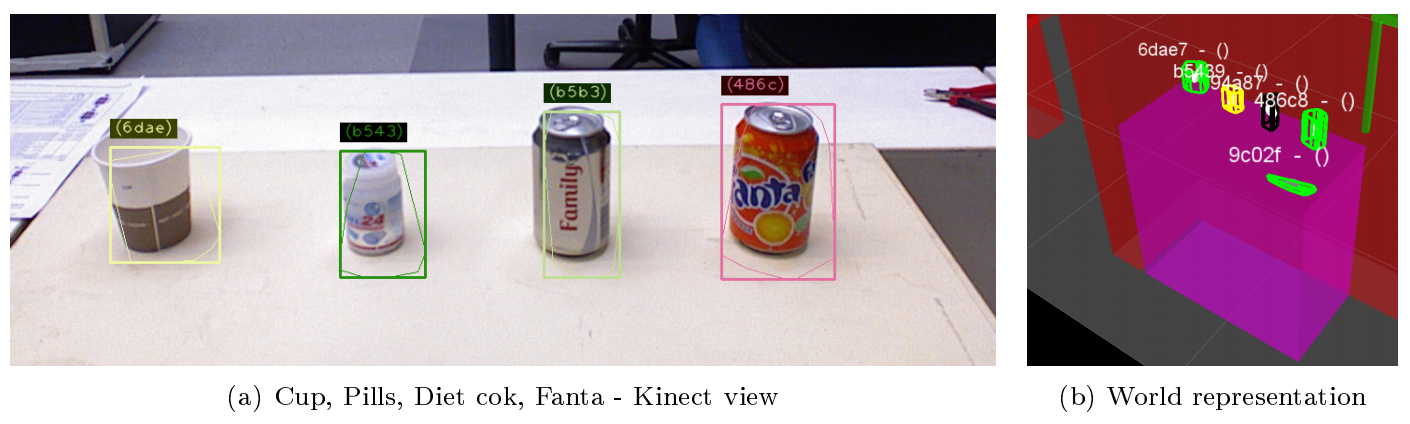
\includegraphics[width = 1\linewidth]{Figures/ed_perception}
    %\vspace{-1em}
    \caption{ED Perception responsible for the object segmentation and calling the object recognition service. Left, the segmented objects in the robot's sensor frame are displayed; the final annotated world representation is shown at the right picture.}
	\label{fig:ed_perception}
    %\vspace{-0.5cm}
\end{figure}

\subsubsection{Recognition using Deep Learning}
In order the classify or train unknown entities, the ed\_perception plugin\footnote{\url{https://github.com/tue-robotics/ed_perception}} exposes ROS Services to classify the entities in the world model. The ed\_perception module interfaces with various image\_recognition nodes that apply state of the art image classification techniques based on \acrfull{cnn} illustrated in Figure \ref{fig:cnn}.
\begin{figure}[h]
    \centering
    %\vspace{-0.3cm}
	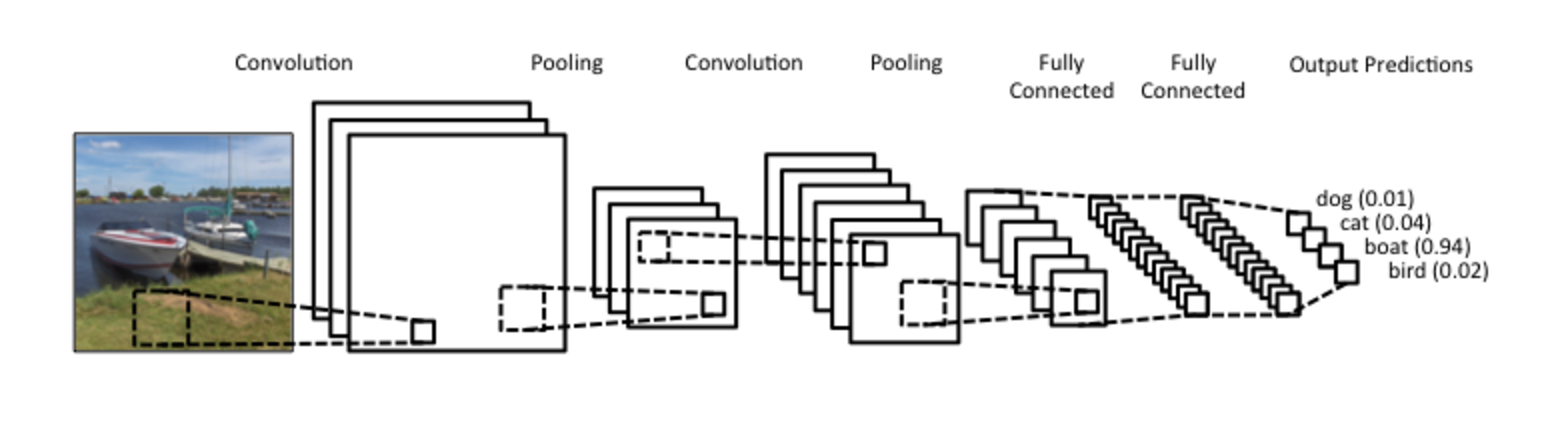
\includegraphics[width = 1\linewidth]{Figures/cnn}
    %\vspace{-1em}
    \caption{Illustration \acrfull{cnn} used in our object recognition nodes with use of Tensorflow.}
	\label{fig:cnn}
    %\vspace{-0.5cm}
\end{figure}
Object recognition is done using Tensorflow: retraining the top-layer of a Inception V3 neural network. The top layers are retrained on a custom dataset using a soft-max top-layer that maps the image representation on a specified set of labels.
\\
Face detection and recognition is done using Openface based on Torch. Openface is an existing state-of-the-art face recognition library. We implemented a ROS node that enables the use of these advanced technologies within the ROS network.
\\\newline
In order to create a new training set for specific objects, the ed\_perception and the image\_recognition packages contains several tools for segmenting and annotating object. Also tools for retraining neural networks are included.
\\
Our image recognition ROS packages can be found at GitHub\footnote{\url{https://github.com/tue-robotics/image_recognition}} with tutorials and documentation. Recently, they have also been added to the ROS Kinetic package list and can be installed as Debian packages:

\begin{lstlisting}
sudo apt install ros-kinetic-image-recognition
\end{lstlisting}